\documentclass[tikz]{standalone}
\input{../tikz/plots_config.pgs}

\begin{document}

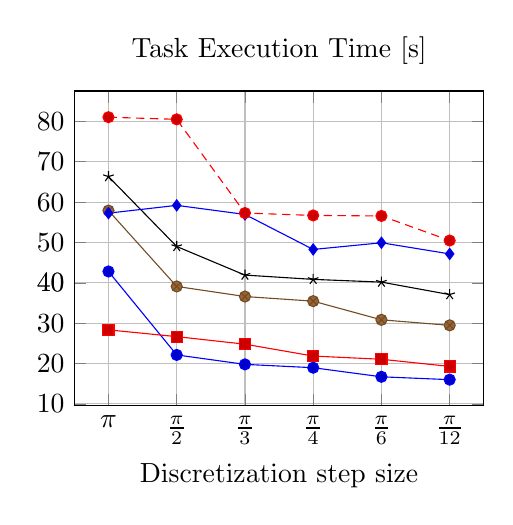
\begin{tikzpicture}
\begin{axis}[%
width=52mm,
height=40mm,
scale only axis,
xmajorgrids,
ymajorgrids,
xtick={1,2,3,4,5,6},
xticklabels={$\pi$,$\frac{\pi}{2}$,$\frac{\pi}{3}$,$\frac{\pi}{4}$,
                                            $\frac{\pi}{6}$, $\frac{\pi}{12}$},
ytick={10, 20, 30, 40, 40, 50, 60, 70, 80},
title={Task Execution Time [s]},
xlabel={Discretization step size},
]
%  n=25
\addplot coordinates{
(1, 42.8010657423)
(2, 22.1163103818)
(3, 19.7736700358)
(4, 18.9472660486)
(5, 16.6927278718)
(6, 15.9834984112)
};

%  n=50
\addplot coordinates{
(1, 28.3284721252)
(2, 26.6475329041)
(3, 24.779245366)
(4, 21.8354147047)
(5, 21.0404409435)
(6, 19.2613158606)
};

%  n=100
\addplot coordinates{
(1, 57.8925354601)
(2, 39.0950969841)
(3, 36.5912972049)
(4, 35.441645496)
(5, 30.8193046648)
(6, 29.4475904746)
};

%  n=150
\addplot coordinates{
(1, 66.3232971495)
(2, 48.9946332404)
(3, 41.9066881984)
(4, 40.8434635126)
(5, 40.16484337)
(6, 37.0715949639)
};

%  n=200
\addplot coordinates{
(1, 57.2575984769)
(2, 59.1927722301)
(3, 56.9417183056)
(4, 48.2612611198)
(5, 49.915562135)
(6, 47.1566786794)
};

%  n=245
\addplot coordinates{
(1, 81.045975235)
(2, 80.5149720494)
(3, 57.2905222519)
(4, 56.6949338939)
(5, 56.567817929)
(6, 50.47492417)
};

\end{axis}
\end{tikzpicture}

\end{document}
